\documentclass[12pt]{scrartcl}
\usepackage{graphicx}
\graphicspath{{./}}
\usepackage[sexy]{evan}
\usepackage[normalem]{ulem}
\usepackage{hyperref}
\usepackage{mathtools}
\usepackage{multicol}
\hypersetup{
    colorlinks=true,
    linkcolor=blue,
    filecolor=magenta,      
    urlcolor=cyan,
    pdfpagemode=FullScreen,
    }
\usepackage[most]{tcolorbox}
\renewcommand{\dangle}{\measuredangle}

\renewcommand{\baselinestretch}{1.5}

\addtolength{\oddsidemargin}{-0.4in}
\addtolength{\evensidemargin}{-0.4in}
\addtolength{\textwidth}{0.8in}
% \addtolength{\topmargin}{-0.2in}
% \addtolength{\textheight}{1in} 


\setlength{\parindent}{0pt}

\usepackage{pgfplots}
\pgfplotsset{compat=1.15}
\usepackage{mathrsfs}
\usetikzlibrary{arrows}

\title{WMI Final 2024 - Simulation 1}
\author{Question Paper}
\date{17.00 WIB, 2 July 2024 - 23.59 WIB, 5 July 2024}

\begin{document}
\maketitle
\begin{center}
    \Huge
    \boxed{\textbf{Grade 5 - 6}}
\end{center}
\vspace{3cm}

\begin{flushleft}
\LARGE
   Total time allowed: 90 minutes\\
\large
   Section A : 40 minutes\\
   Break : 10 minutes\\
   Section B : 40 minutes
\end{flushleft}

\vspace{2cm}
\begin{flushleft}
    \Large
    \textbf{Link to submit the answers:} \url{https://forms.gle/aoH9WRhBWZ3RocXcA}
\end{flushleft}

\newpage
\section*{Simulation Rules}

\begin{enumerate}[leftmargin=*]
    \item There will be \textbf{NO Zoom meetin}g for this simulation. Students are going to do it by themselves.
    
    \item Question papers are going to be uploaded to Google Drive, under folder ''Simulation'' at around 4-5 PM on the day of the simulation. Students may print or download the question paper.
    
    \item There are 25 questions in total.
    \begin{itemize}
        \item Section A consists of 15 Multiple Choice Questions. Problems 1-10 score 6 points each. Problems 11-15 score 8 points each. No points are deducted for unanswered question or wrong answer.
        \item Section B consists of 10 Open-Ended Questions. They score 10 points each, no points are deducted for unanswered or wrong answer.
    \end{itemize}

    \item \textbf{Total time: 90 minutes} 
    \newline
    Section A : 40 minutes.\\
    Break : 10 minutes \\
    Section B : 40 minutes.
    
    Students are advised to set a timer to ensure the timing is accurate and is according to the actual condition during WMI Finals 2024.
    
    \item In order to have the best simulation experience, students are advised to have necessary stationery, blank papers (to scribble), and bottled water.
    
    \item No calculators, smart watches/digital watches and digital dictionaries are allowed.
    
    \item Submission can be done by filling in Google Forms. The links of the Google Forms are on the 1st pages of each question paper.
    
    \item Students may only submit once. If there are multiple submissions, only the first one will be considered.
    
    \item Please submit the answers by Friday 5 July 2024, 23:59 WIB. Late submissions will still be marked, but not included in the ranking.
    
    \item The scores are going to be announced during the class on Saturday, 6 July 2024.
\end{enumerate}

\pagestyle{plain}
\newpage
\section{Section A}
\subsection*{Problems 1-10. Six points each. Choose the best answer from (A) -- (E).}
\hrulefill
\begin{enumerate}
    \item A 5-digit number 134a4 is a multiple of 9. Which number is also a multiple of 9?
    \begin{multicols}{5}
        \begin{enumerate}[(A)]
            \item 3a125
            \item 853a1
            \item 82a49
            \item aa069
            \item 522a72
        \end{enumerate}
    \end{multicols} \hrulefill

    \item Compute $40 \times \left(1-\dfrac{1}{10}\right)\times \left(1-\dfrac{1}{11}\right)\times \left(1-\dfrac{1}{12}\right) \times \dots \times \left(1-\dfrac{1}{20}\right)$.
    \begin{multicols}{5}
        \begin{enumerate}[(A)]
            \item 40
            \item 20
            \item 18
            \item 10
            \item 9
        \end{enumerate}
    \end{multicols} \hrulefill

    \item The figure is the plan view of Terry's house, and each letter represents the length of that side. If $c = 60$ m, $d = 40$ m, $h = 20$ m, find the perimeter of Terry's house in m.
    \begin{figure}[h]
        \centering
        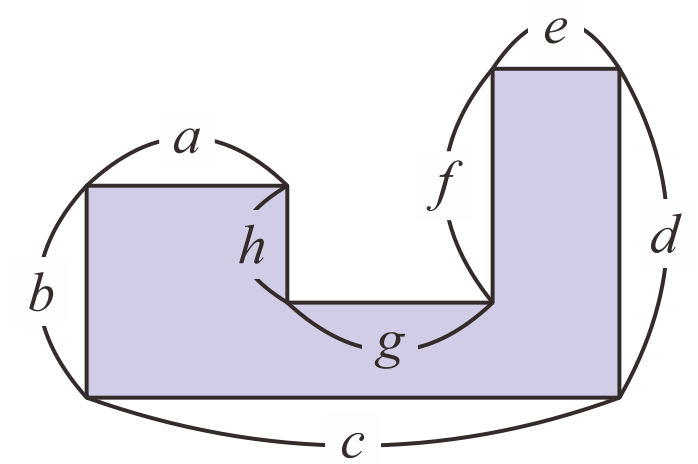
\includegraphics[scale=0.4]{StarGen/0Figure/wmi2023G6A-num3.png}
    \end{figure}
    \begin{multicols}{5}
        \begin{enumerate}[(A)]
            \item 210
            \item 220
            \item 230
            \item 240
            \item 250
        \end{enumerate}
    \end{multicols} \hrulefill

    \item Given a fraction whose denominator is larger than its numerator by 4. If 9 is added to both its numerator and the denominator, and the new fraction can be reduced to $\frac{7}{9}$, find the least common multiple of the numerator and denominator of the original fraction.
    \begin{multicols}{5}
        \begin{enumerate}[(A)]
            \item 21
            \item 77
            \item 36
            \item 90
            \item 45
        \end{enumerate}
    \end{multicols} \hrulefill

    \newpage
    \item Mary uses a 28 cm long bamboo stick to weave a cuboid lantern frame whose length, width, and height are different integers in cm. If rice paper should be stuck on the six faces of the lantern, how much rice paper does she need the least in cm$^2$?
    \begin{multicols}{5}
        \begin{enumerate}[(A)]
            \item 56
            \item 42
            \item 28
            \item 14
            \item 7
        \end{enumerate}
    \end{multicols} \hrulefill

    \item $\dfrac{1}{4} - \dfrac{\square}{2024} = \left(\dfrac{1}{2} + \dfrac{3}{506}\right) \times \dfrac{1}{512}$. Find the sum of the digits in $\square$.
    \begin{multicols}{5}
        \begin{enumerate}[(A)]
            \item 6
            \item 7
            \item 8
            \item 9
            \item 10
        \end{enumerate}
    \end{multicols} \hrulefill

    \item Given a cylinder container, the radius of its bottom surface is 8 cm, its height is 10 cm. Put a cylinder whose radius is 4 cm in the container, fill the container with water, and take the cylinder out of the water. What is the height of the water surface now? ($\pi = 3.14$)
    \begin{figure}[h]
        \centering
        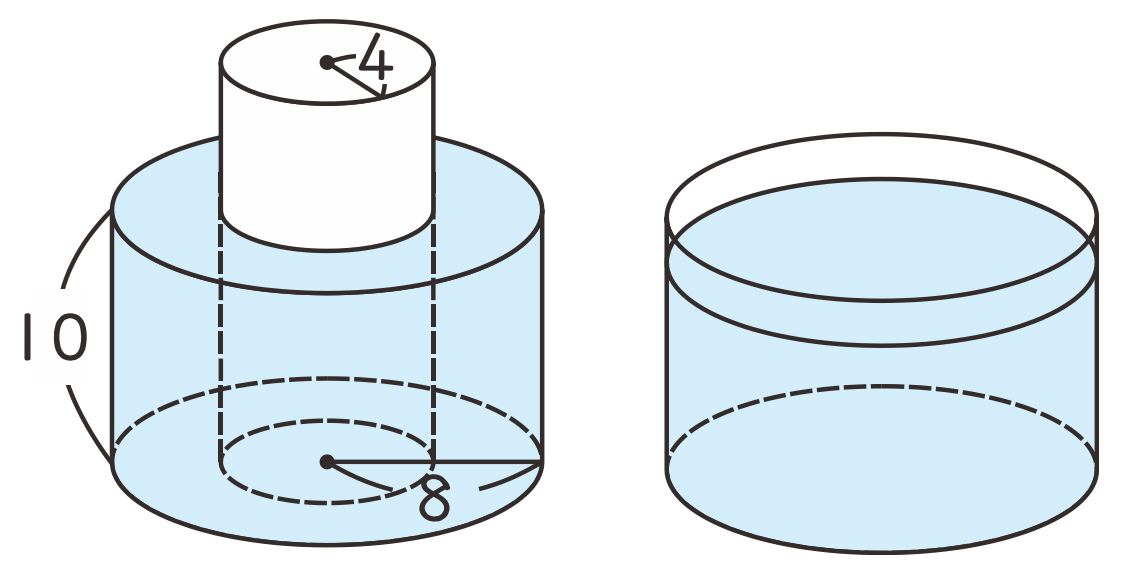
\includegraphics[scale=0.4]{StarGen/0Figure/wmi2023G6A-num7.png}
    \end{figure}
    \begin{multicols}{5}
        \begin{enumerate}[(A)]
            \item 7 cm
            \item 8.5 cm
            \item 7.5 cm
            \item 8 cm
            \item 6.4 cm
        \end{enumerate}
    \end{multicols} \hrulefill

    \item In a juice shop, it is stipulated that each glass of orange juice should contain $\frac{1}{5}$ measuring cup of real juice. A new clerk John mistook $\frac{1}{5}$ for $\frac{1}{4}$. He didn't find out until he'd made 24 glasses of orange juice, and by then there was only $\frac{1}{3}$ of a full bottle of real juice left. If John made orange juice with the correct proportion from the start, how many glasses of orange juice could be made with a full bottle of real juice?
    \begin{multicols}{5}
        \begin{enumerate}[(A)]
            \item 40
            \item 45
            \item 48
            \item 42
            \item 54
        \end{enumerate}
    \end{multicols} \hrulefill

    \newpage
    \item The average number of five numbers is 25. If one of the numbers is changed to 40, and the new average number becomes 30, find the original number of this changed number.
    \begin{multicols}{5}
        \begin{enumerate}[(A)]
            \item 20
            \item 10
            \item 25
            \item 30
            \item 15
        \end{enumerate}
    \end{multicols} \hrulefill

    \item As shown, a path is on a rectangular land which is $x$ m long and $y$ m wide, and the area besides the path is grassland. Move the left sideline of the path rightward horizontally for $k$ m, and it will overlap with the right sideline of the path. If $x:y = 3:2$, $y:k = 4:1$, find the ratio of the area of the path to the area of the grassland.
    \begin{figure}[h]
        \centering
        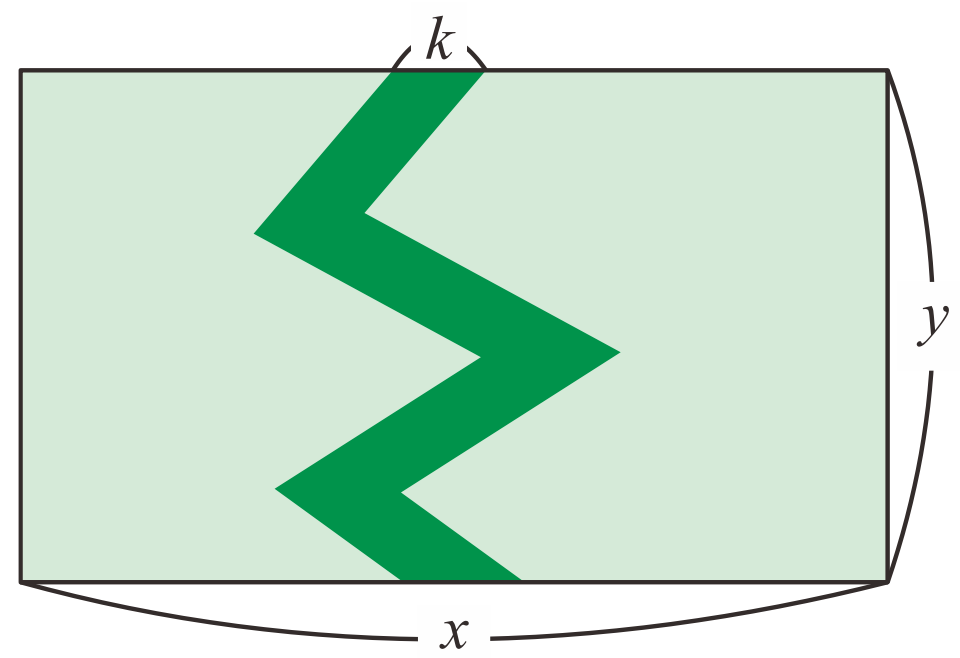
\includegraphics[scale=0.4]{StarGen/0Figure/wmi2023G6A-num8.png}
    \end{figure}
    \begin{multicols}{5}
        \begin{enumerate}[(A)]
            \item $\dfrac{1}{6}$
            \item $\dfrac{1}{12}$
            \item $\dfrac{1}{3}$
            \item $\dfrac{1}{2}$
            \item $\dfrac{2}{5}$
        \end{enumerate}
    \end{multicols} \hrulefill
\end{enumerate}

\subsection*{Problems 11-15. Eight points each. Choose the best answer from (A) -- (E).}
\hrulefill
\begin{enumerate}\setcounter{enumi}{10}
    \item The result of a math test of a class is as follows: The lowest score is 60, the highest score is 100. The score of each student is either a multiple of 2 or 3, and that no two students have the same score. How many students are there in this class at most?
    \begin{multicols}{5}
        \begin{enumerate}[(A)]
            \item 29
            \item 34
            \item 32
            \item 28
            \item 26
        \end{enumerate}
    \end{multicols} \hrulefill

    \newpage
    \item In the left figure is a cuboid water container which is 25 cm long, 10 cm wide, and 24 cm high with a partition that is 10 cm long and 1 cm thick inside. Turn on the tap to fill the container with water, and $x$ minutes later the container is full. In the right figure shows the line chart of the water surface height and the water filling time. Find $x$.
    \begin{figure}[h]
        \centering
        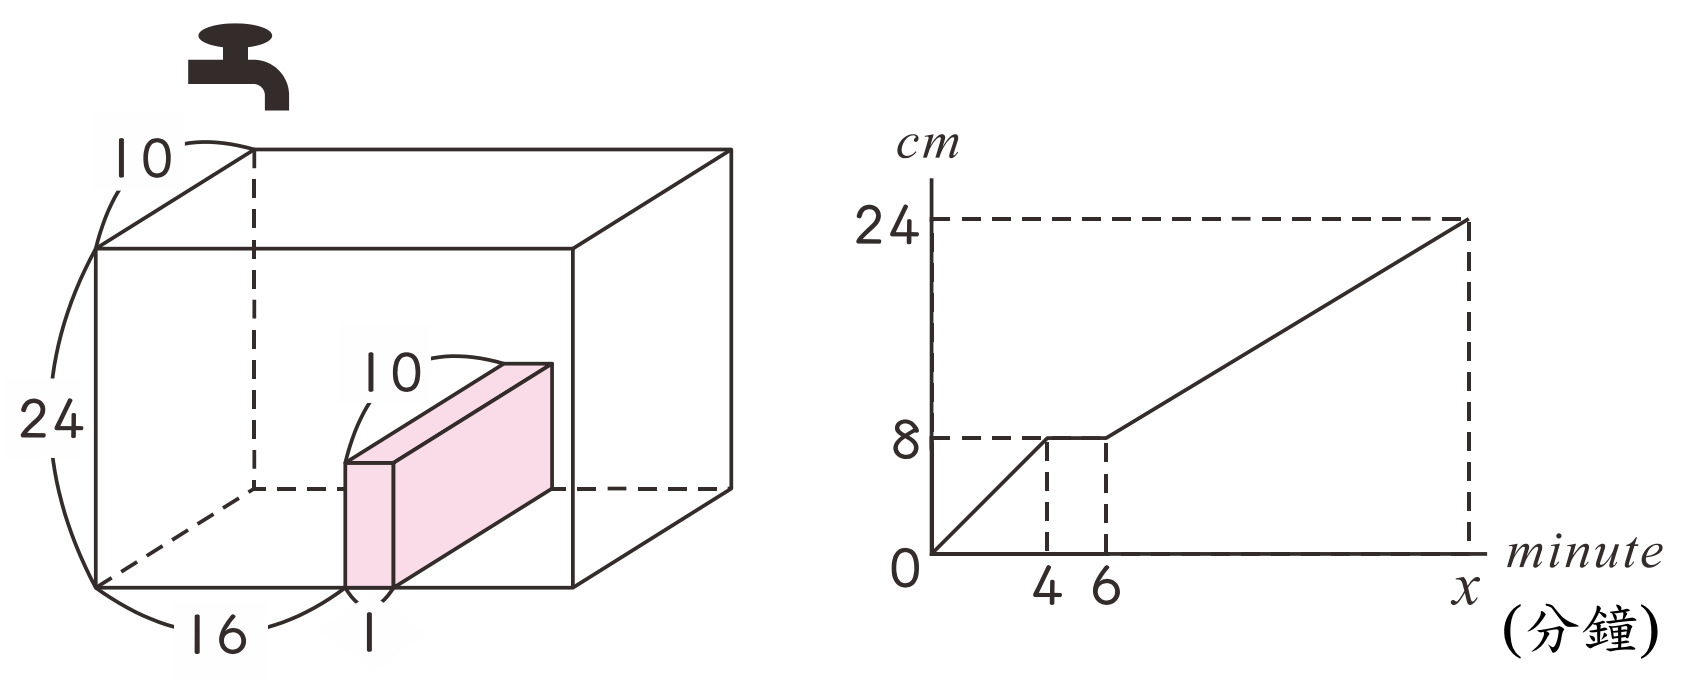
\includegraphics[scale=0.4]{StarGen/0Figure/wmi2023G6A-num11.png}
    \end{figure}
    \begin{multicols}{5}
        \begin{enumerate}[(A)]
            \item 18.6
            \item 18
            \item 18.2
            \item 18.5
            \item 19
        \end{enumerate}
    \end{multicols} \hrulefill

    \item In a rectangular grid, the length and width of each rectangle are 2 and 1, respectively. Suppose two points A and B are on grid points, point C is also on a grid point, and the area of the triangle whose vertices are points A, B, and C is 1, how many points C satisfy the conditions above?
    \begin{figure}[h]
        \centering
        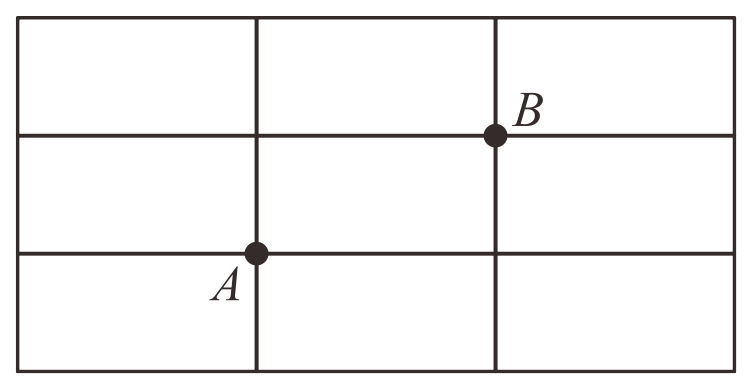
\includegraphics[scale=0.4]{StarGen/0Figure/wmi2023G6A-num12.png}
    \end{figure}
    \begin{multicols}{5}
        \begin{enumerate}[(A)]
            \item 2
            \item 3
            \item 4
            \item 5
            \item 6
        \end{enumerate}
    \end{multicols} \hrulefill

    \newpage
    \item In square ABCD, the area of $\triangle ABE = $ the area of $\triangle BCF = \frac{1}{6}$ of the area of square ABCD. Find the ratio of the area of $\triangle BEF$ to the area of square ABCD.
    \begin{figure}[h]
        \centering
        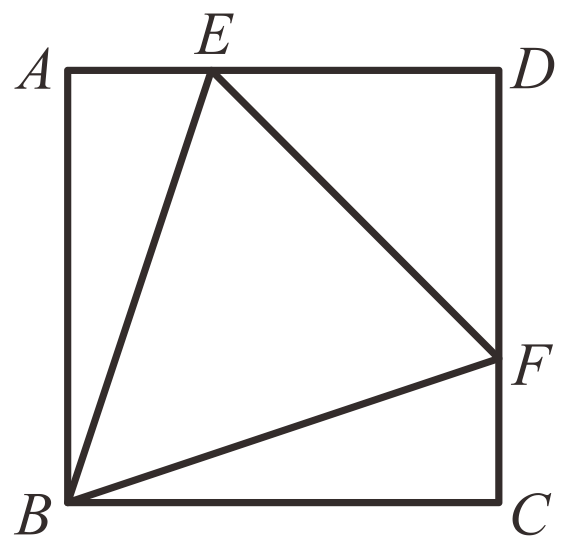
\includegraphics[scale=0.4]{StarGen/0Figure/wmi2023G6A-num15.png}
    \end{figure}
    \begin{multicols}{5}
        \begin{enumerate}[(A)]
            \item $\dfrac{1}{2}$
            \item $\dfrac{2}{5}$
            \item $\dfrac{4}{9}$
            \item $\dfrac{5}{12}$
            \item $\dfrac{7}{18}$
        \end{enumerate}
    \end{multicols} \hrulefill

    \item A circular table symbolizes equality. 6 people sit around a circular table whose radius is 60cm at equal distance from each other. Each person sits 20 cm away from the table. When 2 people join them, each of them moves $x$ cm backward and adjusts their seat leftward or rightward so that each part of the arc length among 8 people is the same as each part of the arc length among 6 people originally. Which equation is appropriate?
    \begin{figure}[h]
        \centering
        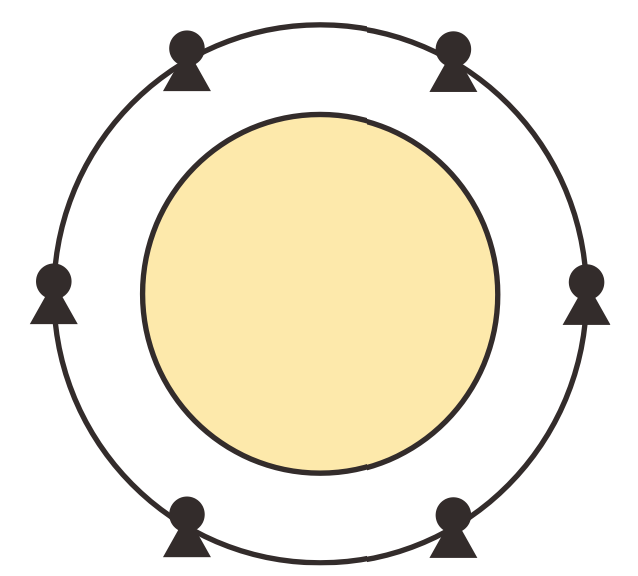
\includegraphics[scale=0.4]{StarGen/0Figure/wmi2023G6A-num13.png}
    \end{figure}
        \begin{enumerate}[(A)]
            \item $\dfrac{2\pi(60+20)}{6} = \dfrac{2\pi(60+20-x)}{8}$
            \item $\dfrac{2\pi \times 60}{6} = \dfrac{2\pi(60+x)}{8}$
            \item $2\pi(60+20) \times 6 = 2\pi(60+20+x) \times 8$
            \item $2\pi(60-x) \times 8 = 2\pi(60+x) \times 6$
            \item $\dfrac{2\pi(60+20)}{6} = \dfrac{2\pi(60+20+x)}{8}$
        \end{enumerate} \hrulefill
\end{enumerate}

\newpage
\section{Section B}
\subsection*{Ten points each. \textbf{No need to write down any units.} All answers are guaranteed in integer form.}
\hrulefill %linefill
\begin{enumerate}[resume]
    \item A positive integer $n$ is a perfect square as well as a multiple of 2023. Find the smallest possible value of $n$.

    \hrulefill \item A bag contains balls of three colors: red, yellow, and blue. If the number of blue balls is $\frac{1}{2}$ of the number of yellow balls at most, the number of blue balls is $\frac{1}{3}$ of the number of red balls at least, and the number of yellow balls and blue balls is not exceeding 100, how many red balls are there in the bag at most?

    \hrulefill \item Given a 3-digit number ABC. Add a 6 to its left, and 6ABC is a multiple of 6. Add a 7 to its right, and ABC7 is a multiple of 7. Add an 8 to its left, and 8ABC is a multiple of 8. Add a 9 to its right, and ABC9 is a multiple of 9. Find the value of ABC.

    \hrulefill \item The circumference of circle O is 720 cm. Moving points A and B start off from point P at the same time and move towards different directions along the circumference. Given that point A moves at the speed of 30 cm/sec, point B moves at the speed of 40 cm/sec. If $x$ seconds after the points move, O, A, and B are on a straight line for the first time, and $y$ seconds after the points move, P, A, and B form an isosceles triangle for the second time, find the value of $70 \times (x + y)$.
    \begin{figure}[h]
        \centering
        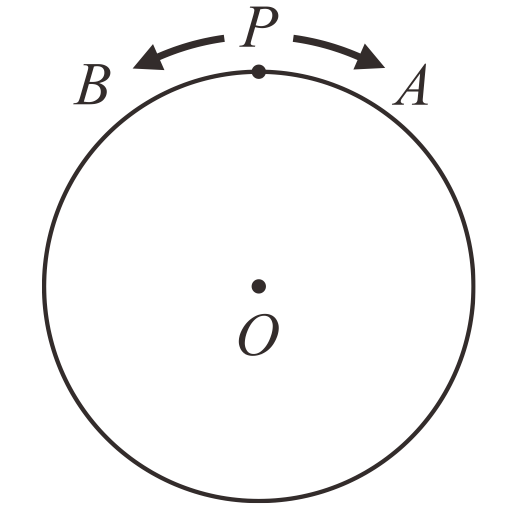
\includegraphics[scale=0.4]{StarGen/0Figure/wmi2023G6B-num4.png}
    \end{figure}

    \hrulefill \item Cut a piece from the cube to make it a heptahedron. If Rachel wants to paint the seven faces with two colors red and blue, how many different ways are there to paint them? (If the solids look the same after rotation or flipping, they are painted in the same way)
    \begin{figure}[h]
        \centering
        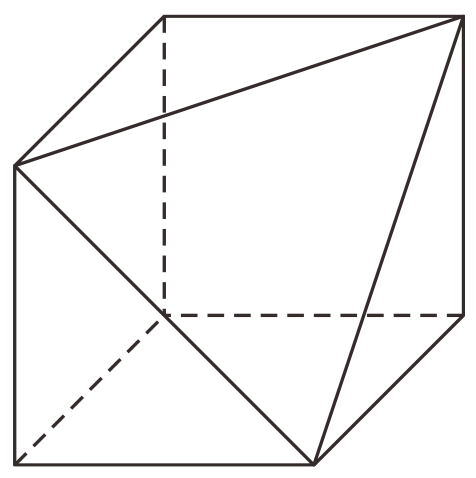
\includegraphics[scale=0.4]{StarGen/0Figure/wmi2023G6B-num5.png}
    \end{figure}

    \hrulefill \item In the equation below, different letters represent different numbers 0--9. Find ABC + DEF.
    \[ (AB - C) \times (DE - F) \times (G + H + I) \times J = 2023 \]

    \hrulefill \item A square is divided into five rectangles with the same area. Given that one of the rectangles is 4 cm wide, find $100x$ in cm.
    \begin{figure}[h]
        \centering
        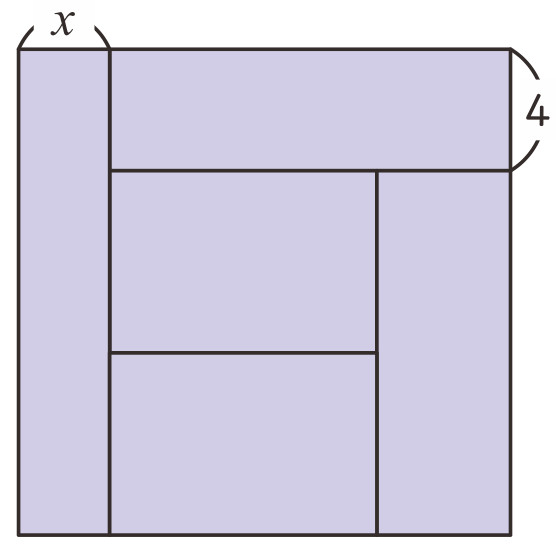
\includegraphics[scale=0.4]{StarGen/0Figure/wmi2023G6B-num7.png}
    \end{figure}

    \hrulefill \item Suppose the units digit of $1^2 + 2^2 + 3^2 + \cdots + 2023^2$ is $x$, and define a new arithmetic operation $a \circ b = \dfrac{a \times b + 4}{a + 2}$. Find $2023 \circ 2022 \circ 2021 \circ \cdots \circ x \circ (x-1) \circ (x-2)$.

    
    \hrulefill
    
    \newpage
    \item The area of parallelogram ABCD is 100 cm$^2$, and the area of pentagon PQRST is 8 cm$^2$. Find the area of the shaded region in cm$^2$.
    \begin{figure}[h]
        \centering
        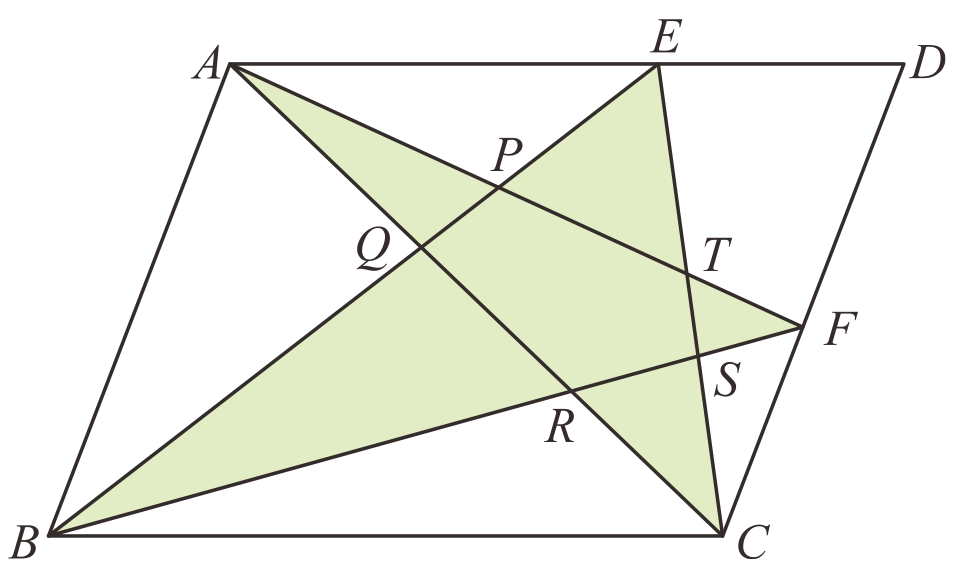
\includegraphics[scale=0.4]{StarGen/0Figure/wmi2023G6B-num9.png}
    \end{figure}

    \hrulefill \item Fill 1-25 in a $5 \times 5$ grid without repetition to make the sum of the numbers in each row, column, and diagonal in the $5 \times 5$ grid and the colored $3 \times 3$ grid the same. Find the multi-digit number ABCD. (Ex: A = 15, B = 3, C = 22, D = 1, ABCD $\rightarrow$ 153221)
    \begin{figure}[h]
        \centering
        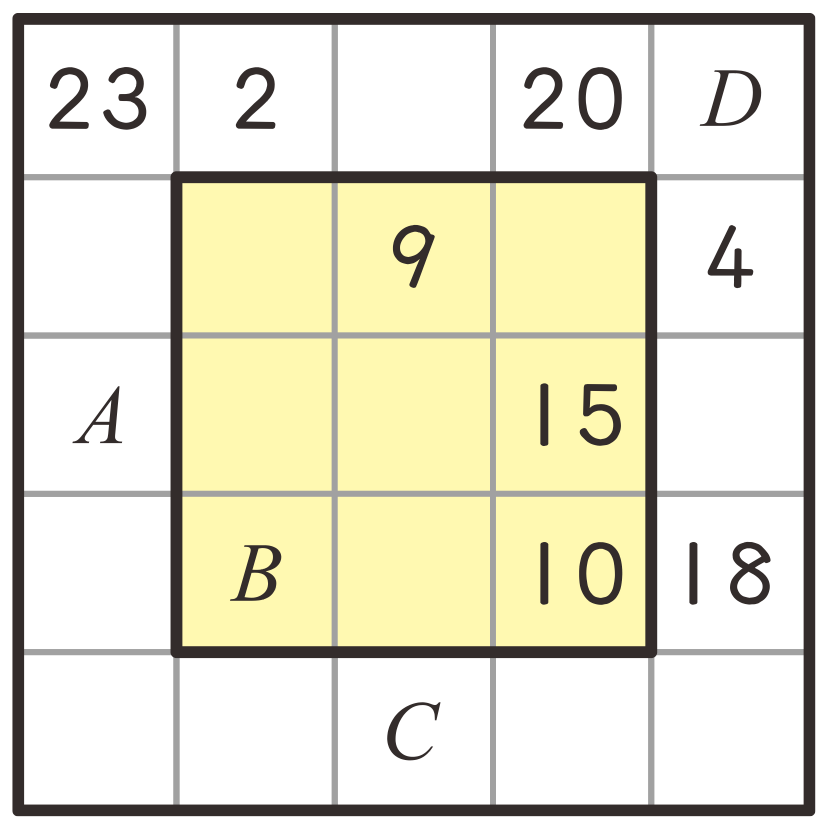
\includegraphics[scale=0.4]{StarGen/0Figure/wmi2023G6B-num10.png}
    \end{figure}

    \hrulefill
\end{enumerate}

\end{document}